\section{Keystone Enclave}
%todo modificare questa intro
Device manufacturers are now taking security concerns more seriously than they previously did as a result of the rise in the popularity of networked devices in recent years.
To adequately address these challenges, Trusted Execution Environments have been developed that define a way to ensure the integrity and confidentiality of sensitive data in the device that implements the specification \cite{IntroTEE}. Keystone \cite{lee2020keystone} is an open-source framework for creating RISC-V hardware-based Trusted Execution Environments that are adaptable for use on a variety of platforms. 

\subsection{Trusted Execution Environment}
A Trusted Execution Environment (TEE) is a safe area within a CPU. It runs in an isolated environment and in parallel with the operating system.
It ensures that the confidentiality and integrity of the code and data loaded in the TEE are preserved. 
Trusted applications running on TEE have access to the full capabilities of a device's main processor and memory, while hardware isolation shields these components from user-installed apps running in the main operating system. The various included trusted applications are protected from one another by software and cryptographic isolations within the TEE \cite{IntroTEE}.
The two most common TEE implementations at the moment are ARM TrustZone and Intel SGX. All these TEEs make design decisions based on either the target applications or threat models and these choices are fixed since they are strictly hardware related. They were not designed to have flexibility or extensibility for enclave developers.  If the hardware changes or has a new feature, the enclave developer has to redesign the TEE.
All TEE platforms aim to reduce the enclave's Trusted computing Base, yet they have managed to achieve different degrees of success \cite{keysyone-blog-1}. The Trusted Computing Base (TCB) is a section of the system, it could include hardware, firmware and software, which is responsible for enforcing the security policy of the system \cite{tcb-def}. Additionally, closed-source hardware and microcode implementations make it impossible for a third party to evaluate the security of TEEs.

\subsubsection{Customizable Trusted Execution Environment}
Customizable TEE is the solution to these problems. It has been designed to be flexible, and configurable and to have a small TCB. It has been designed with clear abstractions and a modular programming model which simplifies for others to extend and add features to the TEE. A customizable TEE is Keystone \cite{lee2020keystone}. Three logical actors, such as the manufacturer (who makes the hardware), the platform provider (runs the hardware, such as a cloud provider), and the enclave developer (who writes software that runs in the enclaves), were identified by keystone developers as being a part of the customizable TEE ecosystem. In a customizable TEE, as opposed to a standard TEE, decisions made by all 3 actors together determine the security guarantees offered and the functionalities enabled \cite{keysyone-blog-1}. 
Keystone offers security primitives that can be joined together via the software framework rather than creating a single instance of TEE hardware. The TEE can be modified by the creator of the enclave and the platform provider to suit their threat models or platform configurations. The Keystone project offers a general and formally proven interface for a variety of devices to create an open standard for TEEs. 

\subsection{RISC-V Background}
RISC-V offers several advantages, apart from being open-source, security-oriented primitives have been added that provide efficient isolation, the most notable being Physical Memory Protection (PMP). RISC-V is an evolving and community-driven Instruction Set Architecture (ISA). Keystone can be designed and developed using standard features and the ever-growing world of RISC-V gives Keystone a wide variety of potential platforms and different deployment scenarios to which it can adapt to. \cite{keysyone-blog-2}

\subsubsection{RISC-V Privilieged ISA}
RISC-V \cite{risc-v-spec} has three software privilege levels (in increasing order of capability): user mode (U-mode), supervisor mode (S-mode), and machine mode (M-mode). Only one of the privilege modes can be active on the processor at once.
The active privilege level determines what the software can do while it is running. These are typical applications for each level of privilege:
\begin{itemize}
    \item U-mode: user processes 
    \item S-mode: kernel (including kernel modules and device drivers) or hypervisor
    \item M-mode: bootloader and firmware
\end{itemize}
When the processor is in the highest privilege mode, M-mode, it is in control of all physical resources and interrupts. As with microcode in Complex Instruction Set Computer (CISC) ISAs (such as x86), M-mode is not interruptible and not affected by the interference of lower modes. M-mode is used in Keystone for executing the TCB of the system, the \textit{security monitor} (SM).
\begin{figure}[h!]
    \centering
    \includesvg[inkscapelatex=false, scale=0.40]{./chapters/images/TEE-keystone-vs-x86.svg}
    \caption{Architecture differences between x86 and keystone}
    \label{keystone-vs-x86}
\end{figure}
The following are some advantages of utilizing an M-mode software as the TCB:
\begin{itemize}
    \item Programmability: unlike microcode for x86, in RISC-V M-mode software can be written using pre-existing toolchains and programming languages, such as C. 
    \item Agile Patching: since the TCB is purely software, bugs or vulnerabilities can be patched without updates, which are specific to a particular hardware 
    \item Verifiability: compared to hardware, the software is generally simpler to be formally verified.
\end{itemize}

\subsubsection{Physical Memory Protection}
Physical Memory Protection (PMP) is a strong standard primitive that enables M-mode to control the access to physical memory from lower privileges modes. Keystone requires PMP to implement memory isolation of enclaves.
Only software in M-mode can configure the PMP, which is controlled by a series of control and status registers (CSR) that limit physical memory access to the U-mode and S-mode. Depending on the platform design, PMP entries number can change. 
Since PMP exclusively works on physical addresses, S-mode can continue to support virtual addresses without affecting the security of the system. Even though each processor may implement PMP differently in hardware, the basic guarantees are part of the standard. PMP is used by Keystone Security Monitor to create memory isolation.

\subsection{Keystone overview}
A Keystone-capable system is made up of different modules operating in various privilege modes as shown in figure \ref{keystoneComponents}.

\begin{figure}[h!]
    \centering
    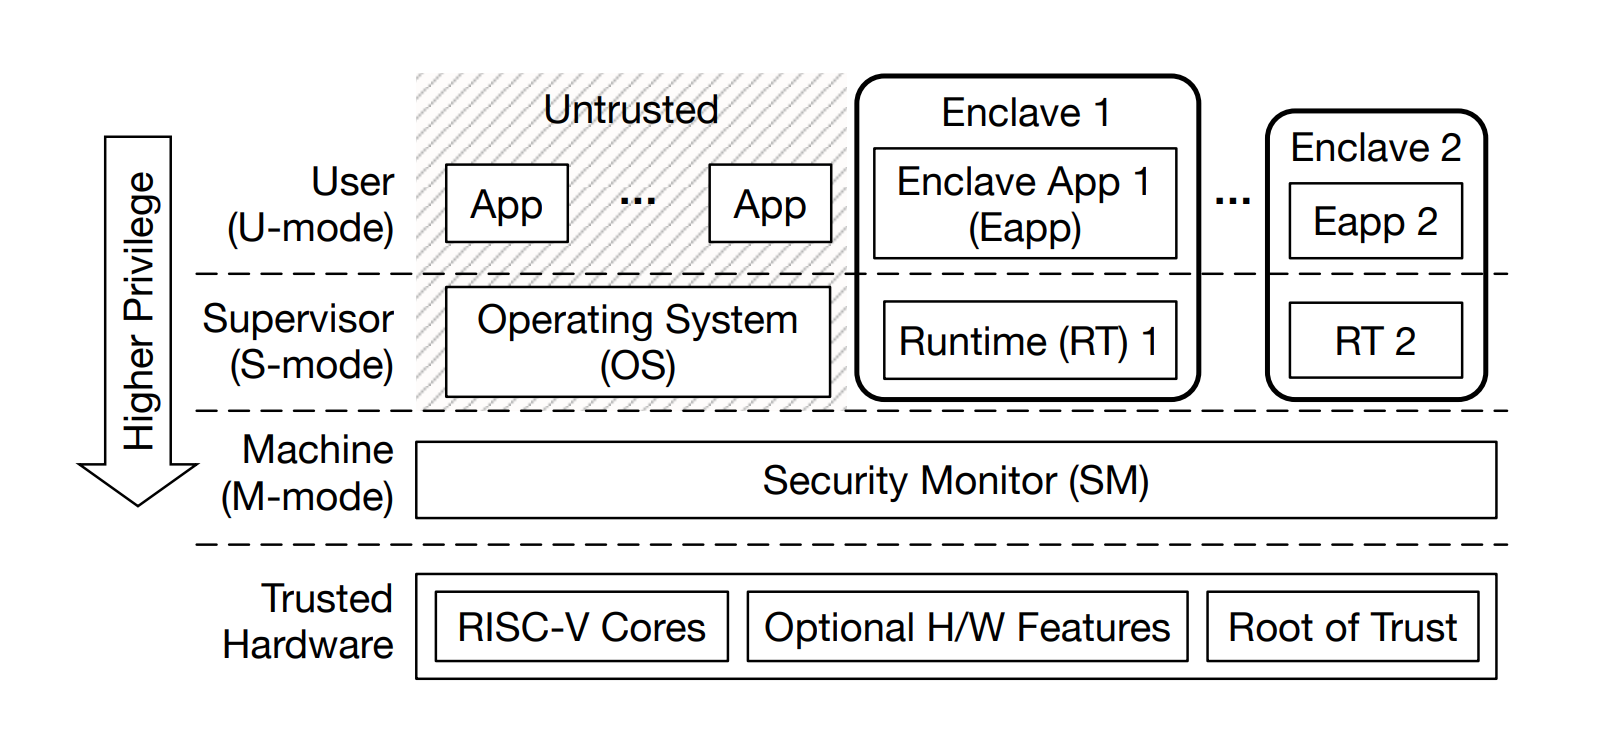
\includegraphics[scale=0.35]{./chapters/images/keystone-components.png}
    \caption{Keystone system with host processes, untrusted OS, security monitor, and multiple enclaves (each with runtime and eapp) \cite{lee2020keystone}.}
    \label{keystoneComponents}
\end{figure}
\subsubsection{Trusted Hardware}
Trusted Hardware is a CPU package built by an honest manufacturer that must enclose standard RISC-V cores that are Keystone compatible and a root of trust. Optional features on the hardware could also include memory encryption, cache partitioning, a cryptographically safe source of randomness, etc. Platform-specific plug-ins are needed by the Security Monitor to support optional features.
\subsubsection{Security Monitor}
Security Monitor (SM) is an M-mode software developed to be a small TCB. The SM serves as an interface for managing the enclave's lifecycle and utilising platform-specific features. The SM manages the isolation boundary between the enclaves and the untrusted OS, therefore it implements the majority of Keystone's security guarantees.
\subsubsection{Runtime}
Runtime is an S-mode software. It implements kernel-like functionality including system calls, trap handling, virtual memory management and so on.
\subsubsection{Enclave}
An Enclave is an environment isolated from the untrusted OS and other enclaves. Each enclave is provided with a private physical memory region which is accessible by only the enclave and SM. Each enclave consists of a user-level enclave application called \textit{eapp} and a supervisor-level runtime. An eapp is a user-level application that executes in the enclave. A developer can create a custom eapp from scratch, or just execute an existing RISC-V binary in Keystone.
